
% ════════════════════════════════════════════
% 模型求解（5.2.4.模型求解.tex，三级子块）
% ════════════════════════════════════════════
\subsubsection{模型求解}

基于上述模型，本节利用附件一与附件二数据逐日求解线性规划，得到全年 365 天的购电与充放电策略。其中 2025 年 1 月作为\textbf{预热期}：模型以 1 月 1 日 0:00 储电量 6000 kWh 为初值逐日滚动，使储电量摆脱初始条件影响、进入稳定的日循环（2 月 1 日 0:00 储电量已收敛至 1200 kWh 下限）；按照附件 5 的要求，结果文件与费用汇总均只统计 2025 年 2 月 1 日至 12 月 31 日（334 天），该口径下购电费用合计为 12254765.72 元，日均约 36690.92 元；由于规划时已知真实负载与光伏，紧急购电量为零。按题目要求，以表1的格式给出表3中四个指定日期在指定时间段的购电量及全天购电量、购电费（表\ref{tab:结果2-1a}～表\ref{tab:结果2-1d}），以表2的格式给出储能设备在指定时间段的充放电量及0:00和24:00储电量（表\ref{tab:结果2-2a}～表\ref{tab:结果2-2d}），并以表3的格式给出紧急购电结果（表\ref{tab:结果2-3}）；由于规划时已知真实负载与光伏，四个指定日期的紧急购电量均为零。

\begin{longtable}{>{\centering\arraybackslash}p{0.15\textwidth}>{\centering\arraybackslash}p{0.13\textwidth}>{\centering\arraybackslash}p{0.15\textwidth}>{\centering\arraybackslash}p{0.13\textwidth}>{\centering\arraybackslash}p{0.15\textwidth}>{\centering\arraybackslash}p{0.13\textwidth}}
  \caption{2025.3.20 微网在指定时间段的购电量及全天的购电量和购电费}
  \label{tab:结果2-1a} \\
  \toprule
  时间段 & 购电量 & 时间段 & 购电量 & 时间段 & 购电量 \\
  \midrule
  \endfirsthead
  \caption{2025.3.20 微网在指定时间段的购电量及全天的购电量和购电费（续）} \\
  \toprule
  时间段 & 购电量 & 时间段 & 购电量 & 时间段 & 购电量 \\
  \midrule
  \endhead
  \bottomrule
  \endfoot
  10:00--10:10 & 0.00 & 12:00--12:10 & 479.31 & 14:00--14:10 & 0.00 \\
  16:00--16:10 & 562.26 & 18:00--18:10 & 698.00 & 20:00--20:10 & 0.00 \\
  全天购电量 & 66322.04 & 全天购电费 & 40020.38 &  &  \\
\end{longtable}

\begin{longtable}{>{\centering\arraybackslash}p{0.15\textwidth}>{\centering\arraybackslash}p{0.13\textwidth}>{\centering\arraybackslash}p{0.15\textwidth}>{\centering\arraybackslash}p{0.13\textwidth}>{\centering\arraybackslash}p{0.15\textwidth}>{\centering\arraybackslash}p{0.13\textwidth}}
  \caption{2025.6.21 微网在指定时间段的购电量及全天的购电量和购电费}
  \label{tab:结果2-1b} \\
  \toprule
  时间段 & 购电量 & 时间段 & 购电量 & 时间段 & 购电量 \\
  \midrule
  \endfirsthead
  \caption{2025.6.21 微网在指定时间段的购电量及全天的购电量和购电费（续）} \\
  \toprule
  时间段 & 购电量 & 时间段 & 购电量 & 时间段 & 购电量 \\
  \midrule
  \endhead
  \bottomrule
  \endfoot
  10:00--10:10 & 0.00 & 12:00--12:10 & 0.00 & 14:00--14:10 & 0.00 \\
  16:00--16:10 & 78.57 & 18:00--18:10 & 0.00 & 20:00--20:10 & 0.00 \\
  全天购电量 & 32057.47 & 全天购电费 & 17599.36 &  &  \\
\end{longtable}

\begin{longtable}{>{\centering\arraybackslash}p{0.15\textwidth}>{\centering\arraybackslash}p{0.13\textwidth}>{\centering\arraybackslash}p{0.15\textwidth}>{\centering\arraybackslash}p{0.13\textwidth}>{\centering\arraybackslash}p{0.15\textwidth}>{\centering\arraybackslash}p{0.13\textwidth}}
  \caption{2025.9.23 微网在指定时间段的购电量及全天的购电量和购电费}
  \label{tab:结果2-1c} \\
  \toprule
  时间段 & 购电量 & 时间段 & 购电量 & 时间段 & 购电量 \\
  \midrule
  \endfirsthead
  \caption{2025.9.23 微网在指定时间段的购电量及全天的购电量和购电费（续）} \\
  \toprule
  时间段 & 购电量 & 时间段 & 购电量 & 时间段 & 购电量 \\
  \midrule
  \endhead
  \bottomrule
  \endfoot
  10:00--10:10 & 0.00 & 12:00--12:10 & 354.19 & 14:00--14:10 & 0.00 \\
  16:00--16:10 & 589.43 & 18:00--18:10 & 764.33 & 20:00--20:10 & 0.00 \\
  全天购电量 & 66265.42 & 全天购电费 & 41395.50 &  &  \\
\end{longtable}

\begin{longtable}{>{\centering\arraybackslash}p{0.15\textwidth}>{\centering\arraybackslash}p{0.13\textwidth}>{\centering\arraybackslash}p{0.15\textwidth}>{\centering\arraybackslash}p{0.13\textwidth}>{\centering\arraybackslash}p{0.15\textwidth}>{\centering\arraybackslash}p{0.13\textwidth}}
  \caption{2025.12.21 微网在指定时间段的购电量及全天的购电量和购电费}
  \label{tab:结果2-1d} \\
  \toprule
  时间段 & 购电量 & 时间段 & 购电量 & 时间段 & 购电量 \\
  \midrule
  \endfirsthead
  \caption{2025.12.21 微网在指定时间段的购电量及全天的购电量和购电费（续）} \\
  \toprule
  时间段 & 购电量 & 时间段 & 购电量 & 时间段 & 购电量 \\
  \midrule
  \endhead
  \bottomrule
  \endfoot
  10:00--10:10 & 0.00 & 12:00--12:10 & 932.83 & 14:00--14:10 & 0.00 \\
  16:00--16:10 & 801.38 & 18:00--18:10 & 715.41 & 20:00--20:10 & 0.00 \\
  全天购电量 & 93770.21 & 全天购电费 & 59747.81 &  &  \\
\end{longtable}

\begin{longtable}{>{\centering\arraybackslash}p{0.15\textwidth}>{\centering\arraybackslash}p{0.13\textwidth}>{\centering\arraybackslash}p{0.13\textwidth}>{\centering\arraybackslash}p{0.15\textwidth}>{\centering\arraybackslash}p{0.13\textwidth}>{\centering\arraybackslash}p{0.13\textwidth}}
  \caption{2025.3.20 储能设备在指定时间段的充放电量及0:00和24:00的储电量}
  \label{tab:结果2-2a} \\
  \toprule
  时间段 & 充电量 & 放电量 & 时间段 & 充电量 & 放电量 \\
  \midrule
  \endfirsthead
  \caption{2025.3.20 储能设备在指定时间段的充放电量及0:00和24:00的储电量（续）} \\
  \toprule
  时间段 & 充电量 & 放电量 & 时间段 & 充电量 & 放电量 \\
  \midrule
  \endhead
  \bottomrule
  \endfoot
  0:00--4:00 & 979.35 & 0.00 & 4:00--8:00 & 833.33 & 1468.27 \\
  8:00--12:00 & 2925.38 & 0.00 & 12:00--16:00 & 7741.29 & 0.00 \\
  16:00--20:00 & 0.00 & 6252.90 & 20:00--24:00 & 0.00 & 2387.10 \\
  0:00储电量 & 1200.00 &  & 24:00储电量 & 1200.00 &  \\
\end{longtable}

\begin{longtable}{>{\centering\arraybackslash}p{0.15\textwidth}>{\centering\arraybackslash}p{0.13\textwidth}>{\centering\arraybackslash}p{0.13\textwidth}>{\centering\arraybackslash}p{0.15\textwidth}>{\centering\arraybackslash}p{0.13\textwidth}>{\centering\arraybackslash}p{0.13\textwidth}}
  \caption{2025.6.21 储能设备在指定时间段的充放电量及0:00和24:00的储电量}
  \label{tab:结果2-2b} \\
  \toprule
  时间段 & 充电量 & 放电量 & 时间段 & 充电量 & 放电量 \\
  \midrule
  \endfirsthead
  \caption{2025.6.21 储能设备在指定时间段的充放电量及0:00和24:00的储电量（续）} \\
  \toprule
  时间段 & 充电量 & 放电量 & 时间段 & 充电量 & 放电量 \\
  \midrule
  \endhead
  \bottomrule
  \endfoot
  0:00--4:00 & 9000.00 & 0.00 & 4:00--8:00 & 1666.67 & 6927.39 \\
  8:00--12:00 & 5154.73 & 1712.61 & 12:00--16:00 & 5604.34 & 74.85 \\
  16:00--20:00 & 0.00 & 5576.93 & 20:00--24:00 & 0.00 & 3063.07 \\
  0:00储电量 & 1200.00 &  & 24:00储电量 & 1200.00 &  \\
\end{longtable}

\begin{longtable}{>{\centering\arraybackslash}p{0.15\textwidth}>{\centering\arraybackslash}p{0.13\textwidth}>{\centering\arraybackslash}p{0.13\textwidth}>{\centering\arraybackslash}p{0.15\textwidth}>{\centering\arraybackslash}p{0.13\textwidth}>{\centering\arraybackslash}p{0.13\textwidth}}
  \caption{2025.9.23 储能设备在指定时间段的充放电量及0:00和24:00的储电量}
  \label{tab:结果2-2c} \\
  \toprule
  时间段 & 充电量 & 放电量 & 时间段 & 充电量 & 放电量 \\
  \midrule
  \endfirsthead
  \caption{2025.9.23 储能设备在指定时间段的充放电量及0:00和24:00的储电量（续）} \\
  \toprule
  时间段 & 充电量 & 放电量 & 时间段 & 充电量 & 放电量 \\
  \midrule
  \endhead
  \bottomrule
  \endfoot
  0:00--4:00 & 9000.00 & 0.00 & 4:00--8:00 & 1666.67 & 6577.11 \\
  8:00--12:00 & 5512.02 & 2062.89 & 12:00--16:00 & 5236.78 & 66.53 \\
  16:00--20:00 & 0.00 & 6336.19 & 20:00--24:00 & 0.00 & 2303.81 \\
  0:00储电量 & 1200.00 &  & 24:00储电量 & 1200.00 &  \\
\end{longtable}

\begin{longtable}{>{\centering\arraybackslash}p{0.15\textwidth}>{\centering\arraybackslash}p{0.13\textwidth}>{\centering\arraybackslash}p{0.13\textwidth}>{\centering\arraybackslash}p{0.15\textwidth}>{\centering\arraybackslash}p{0.13\textwidth}>{\centering\arraybackslash}p{0.13\textwidth}}
  \caption{2025.12.21 储能设备在指定时间段的充放电量及0:00和24:00的储电量}
  \label{tab:结果2-2d} \\
  \toprule
  时间段 & 充电量 & 放电量 & 时间段 & 充电量 & 放电量 \\
  \midrule
  \endfirsthead
  \caption{2025.12.21 储能设备在指定时间段的充放电量及0:00和24:00的储电量（续）} \\
  \toprule
  时间段 & 充电量 & 放电量 & 时间段 & 充电量 & 放电量 \\
  \midrule
  \endhead
  \bottomrule
  \endfoot
  0:00--4:00 & 9000.00 & 0.00 & 4:00--8:00 & 2500.00 & 1508.33 \\
  8:00--12:00 & 5833.33 & 7806.67 & 12:00--16:00 & 7717.70 & 2336.33 \\
  16:00--20:00 & 0.00 & 5737.84 & 20:00--24:00 & 0.00 & 2902.16 \\
  0:00储电量 & 1200.00 &  & 24:00储电量 & 1200.00 &  \\
\end{longtable}

\begin{longtable}{>{\centering\arraybackslash}p{0.11\textwidth}>{\centering\arraybackslash}p{0.08\textwidth}>{\centering\arraybackslash}p{0.11\textwidth}>{\centering\arraybackslash}p{0.08\textwidth}>{\centering\arraybackslash}p{0.11\textwidth}>{\centering\arraybackslash}p{0.08\textwidth}>{\centering\arraybackslash}p{0.11\textwidth}>{\centering\arraybackslash}p{0.08\textwidth}}
  \caption{微网在指定日期的紧急购电量}
  \label{tab:结果2-3} \\
  \toprule
  \multicolumn{2}{c}{2025.3.20} & \multicolumn{2}{c}{2025.6.21} & \multicolumn{2}{c}{2025.9.23} & \multicolumn{2}{c}{2025.12.21} \\
  \cmidrule(lr){1-2} \cmidrule(lr){3-4} \cmidrule(lr){5-6} \cmidrule(lr){7-8}
  时间段 & 购电量 & 时间段 & 购电量 & 时间段 & 购电量 & 时间段 & 购电量 \\
  \midrule
  \endfirsthead
  \caption{微网在指定日期的紧急购电量（续）} \\
  \toprule
  \multicolumn{2}{c}{2025.3.20} & \multicolumn{2}{c}{2025.6.21} & \multicolumn{2}{c}{2025.9.23} & \multicolumn{2}{c}{2025.12.21} \\
  \cmidrule(lr){1-2} \cmidrule(lr){3-4} \cmidrule(lr){5-6} \cmidrule(lr){7-8}
  时间段 & 购电量 & 时间段 & 购电量 & 时间段 & 购电量 & 时间段 & 购电量 \\
  \midrule
  \endhead
  \bottomrule
  \endfoot
  --- & 0.00 & --- & 0.00 & --- & 0.00 & --- & 0.00 \\
\end{longtable}

2.1—12.31 逐日购电费用及其 7 日滑动平均如图\ref{fig:结果2-2}所示。可以看出，购电费呈现明显的季节性波动：冬季（12 月）因光伏出力低、负荷高，购电费最高；夏季（6 月）因光伏出力充沛，购电费最低，与光伏资源的季节规律一致。

\begin{figure}[H]
    \centering
    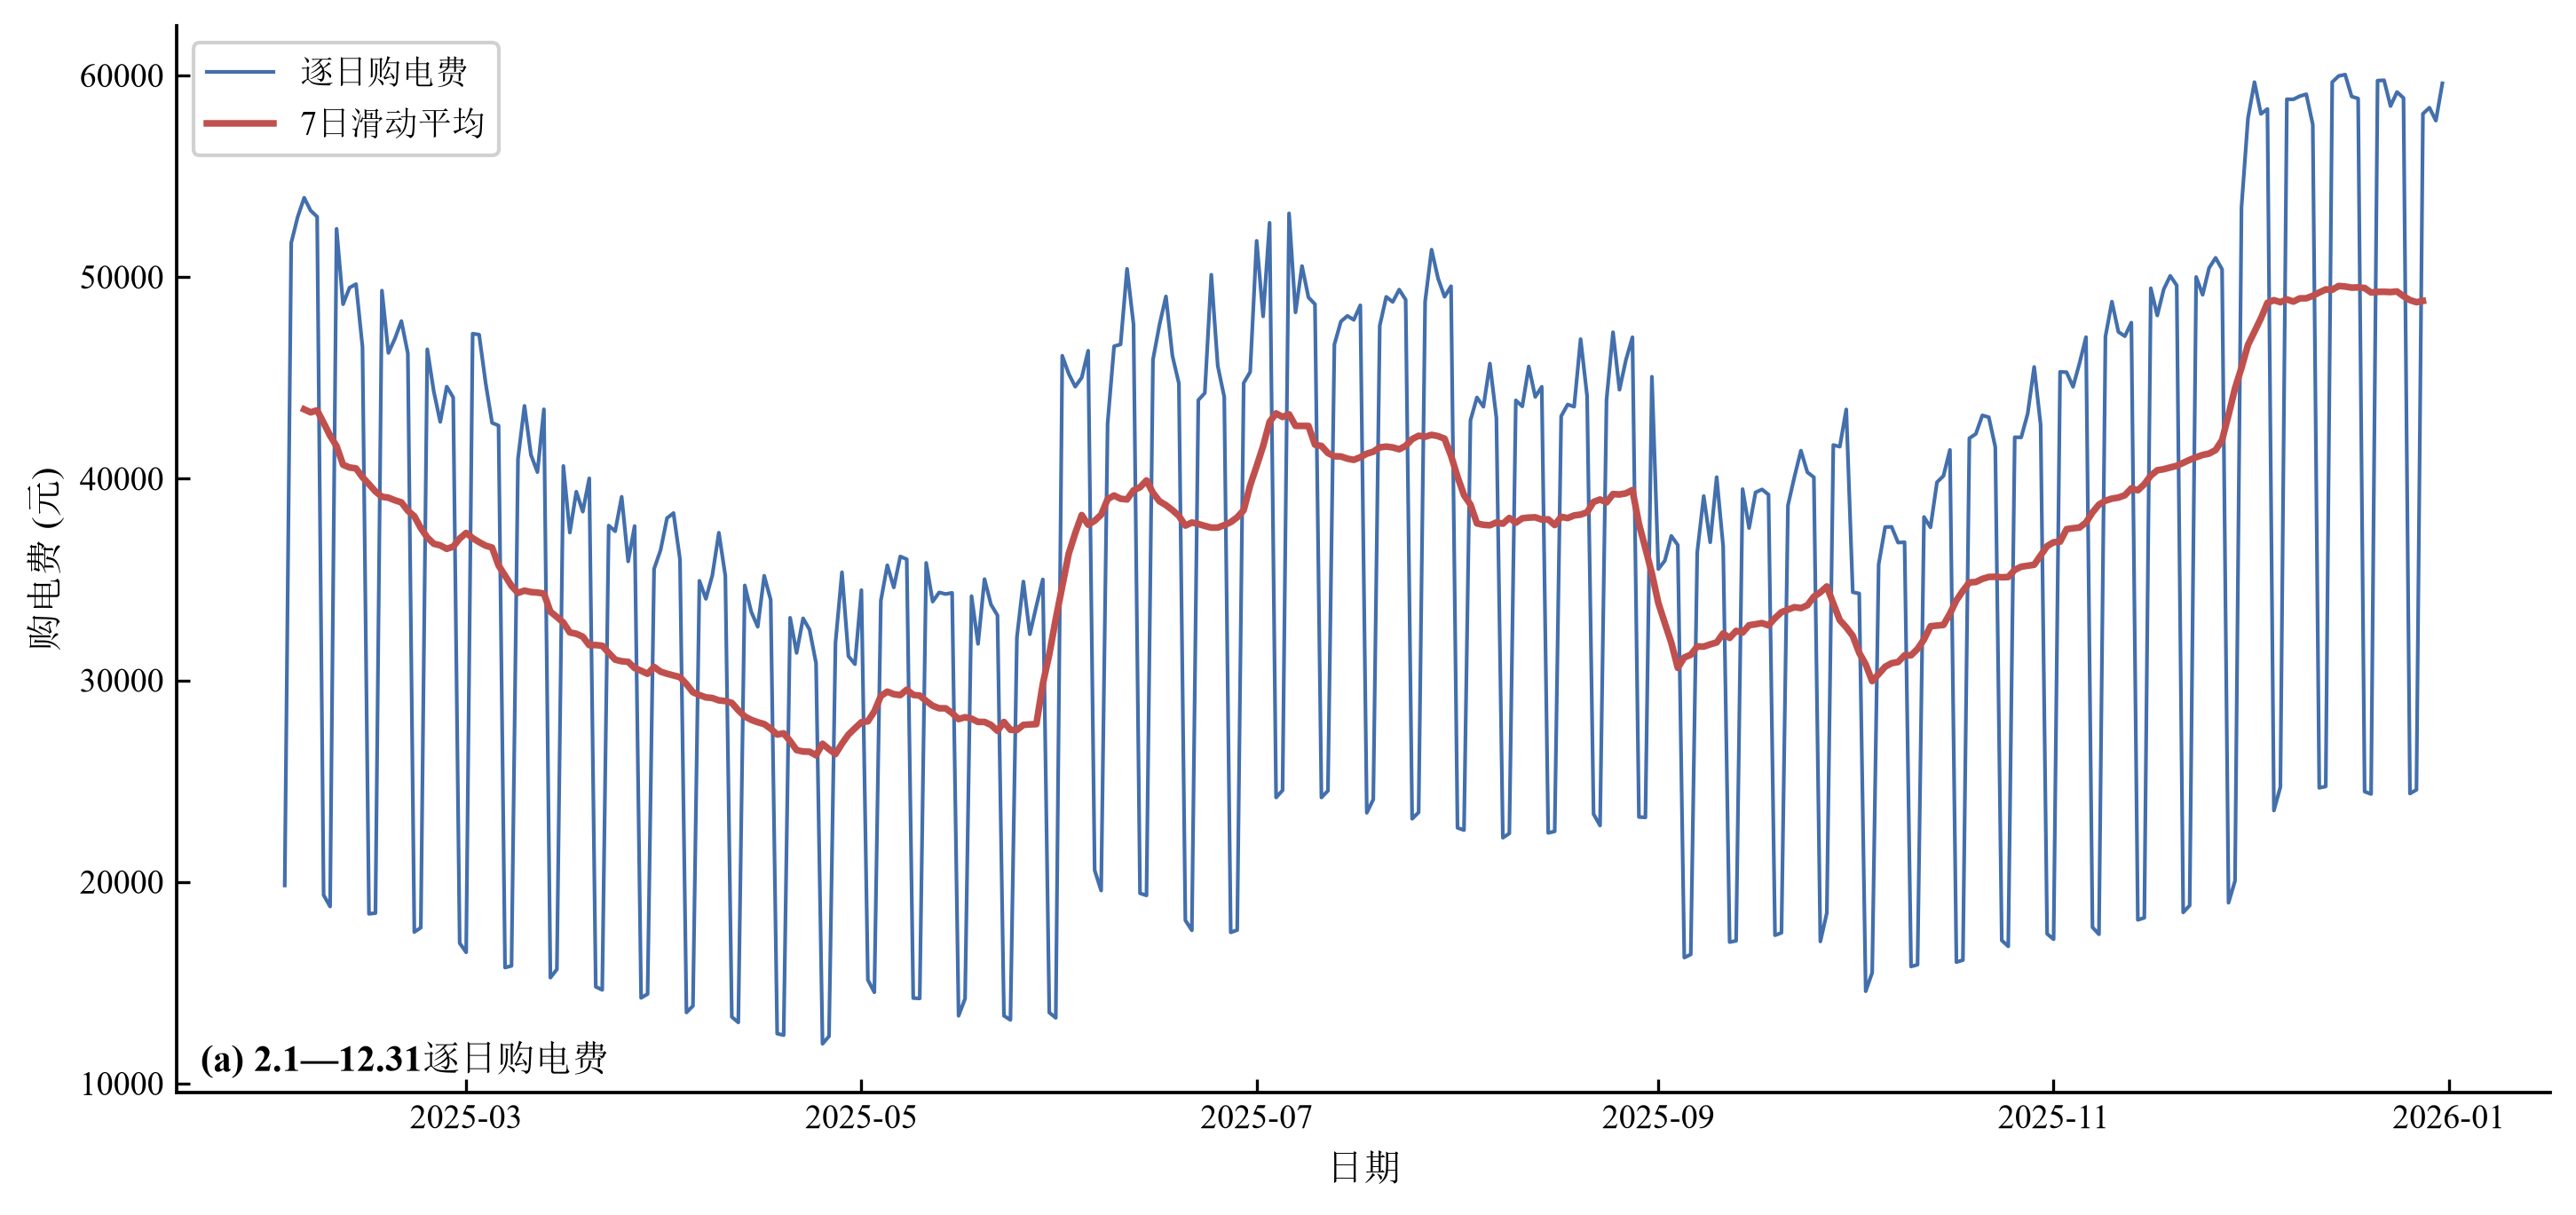
\includegraphics[width=0.70\textwidth]{求解/问题二/图片/图2-2_全年逐日购电费.png}
    \caption{2.1—12.31逐日购电费及7日滑动平均}
    \label{fig:结果2-2}
\end{figure}

四季典型日的购电功率曲线如图\ref{fig:结果2-3}所示。四个季节的购电功率均集中在夜间低电价时段，白天因光伏与储能放电的支撑，购电功率显著减小；冬季典型日购电功率整体最高，与表\ref{tab:结果2-1d}中冬季购电费最高相吻合。

\begin{figure}[H]
    \centering
    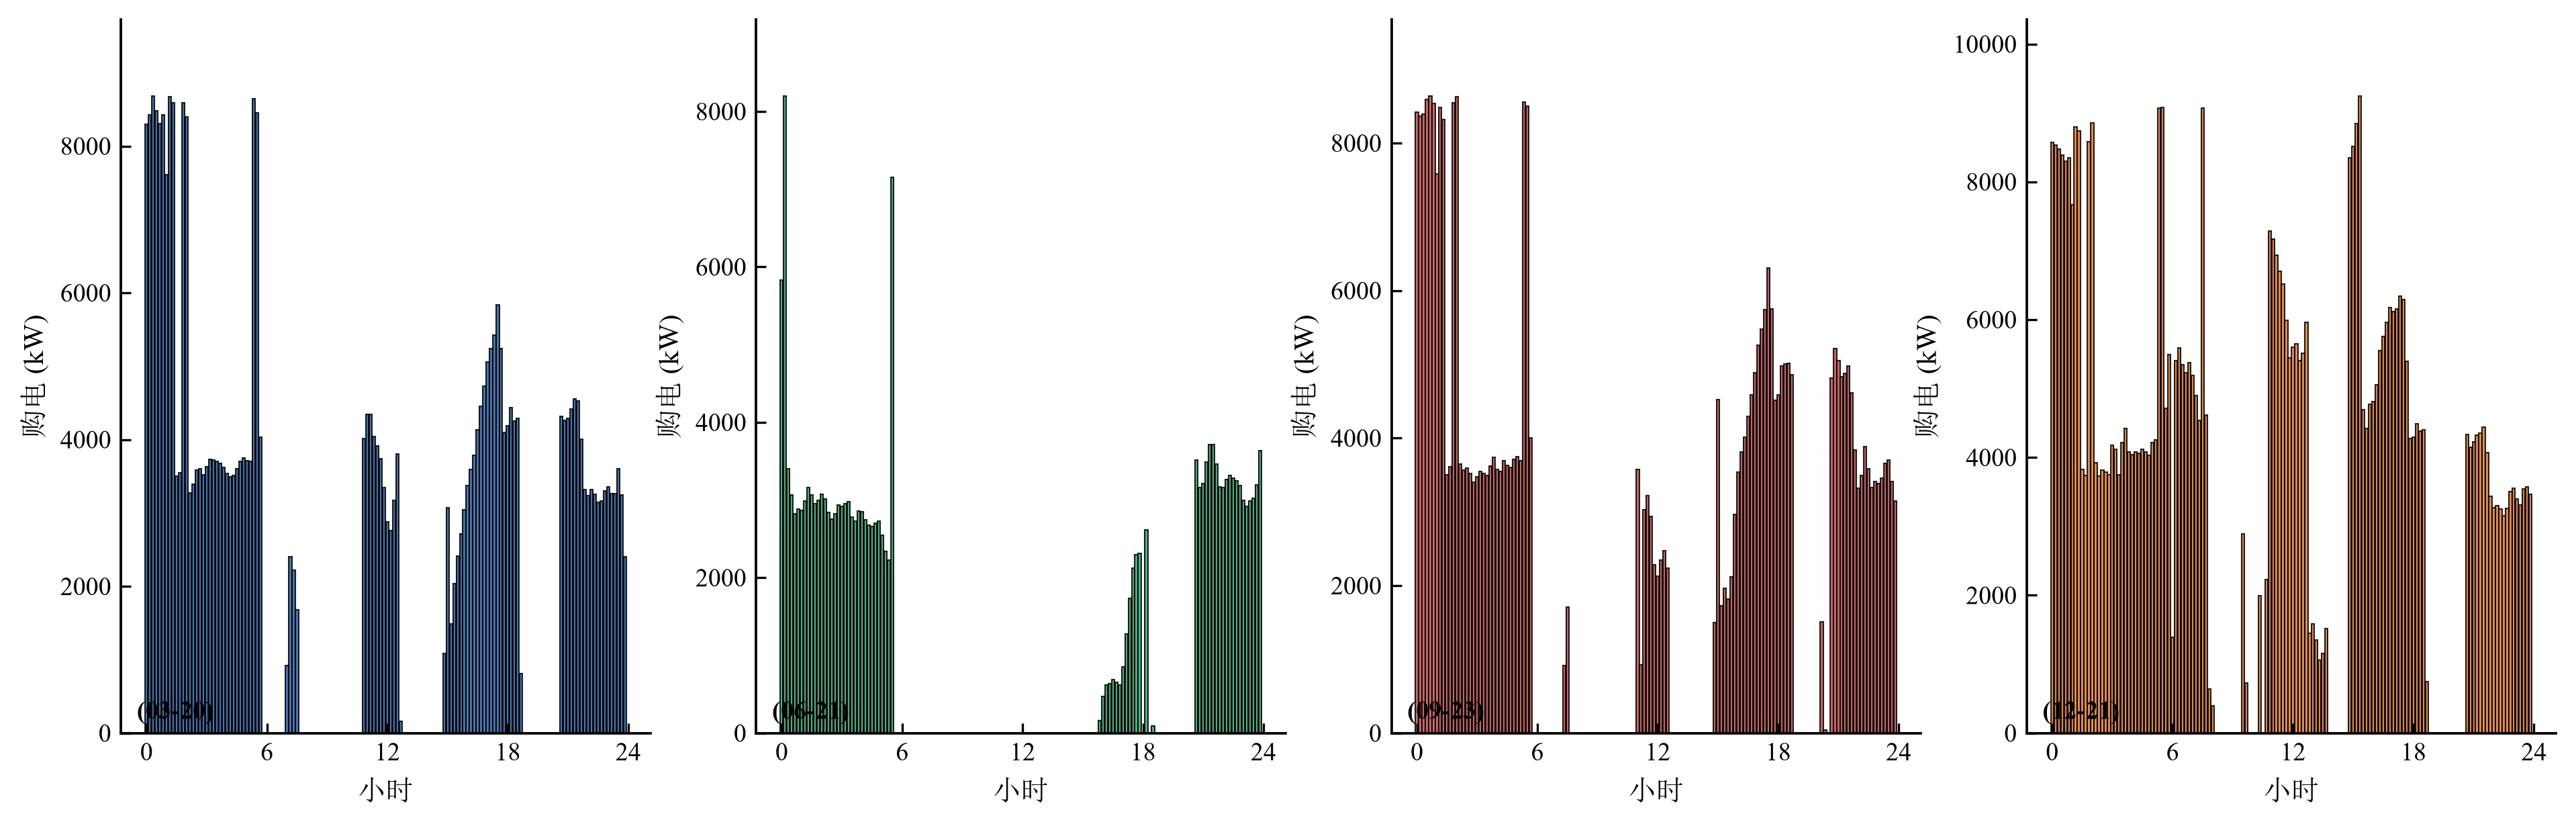
\includegraphics[width=0.75\textwidth]{求解/问题二/图片/图2-3_四季典型日购电策略.png}
    \caption{四季典型日的购电功率策略}
    \label{fig:结果2-3}
\end{figure}

四季典型日的储能荷电状态轨迹如图\ref{fig:结果2-4}所示。储能荷电状态每日在 1200 kWh 与 10800 kWh 之间完成一次充放循环，白天光伏盈余时充电、夜间与傍晚放电，且全天严格处于约束区间内，验证了滚动模型的可行性。

\begin{figure}[H]
    \centering
    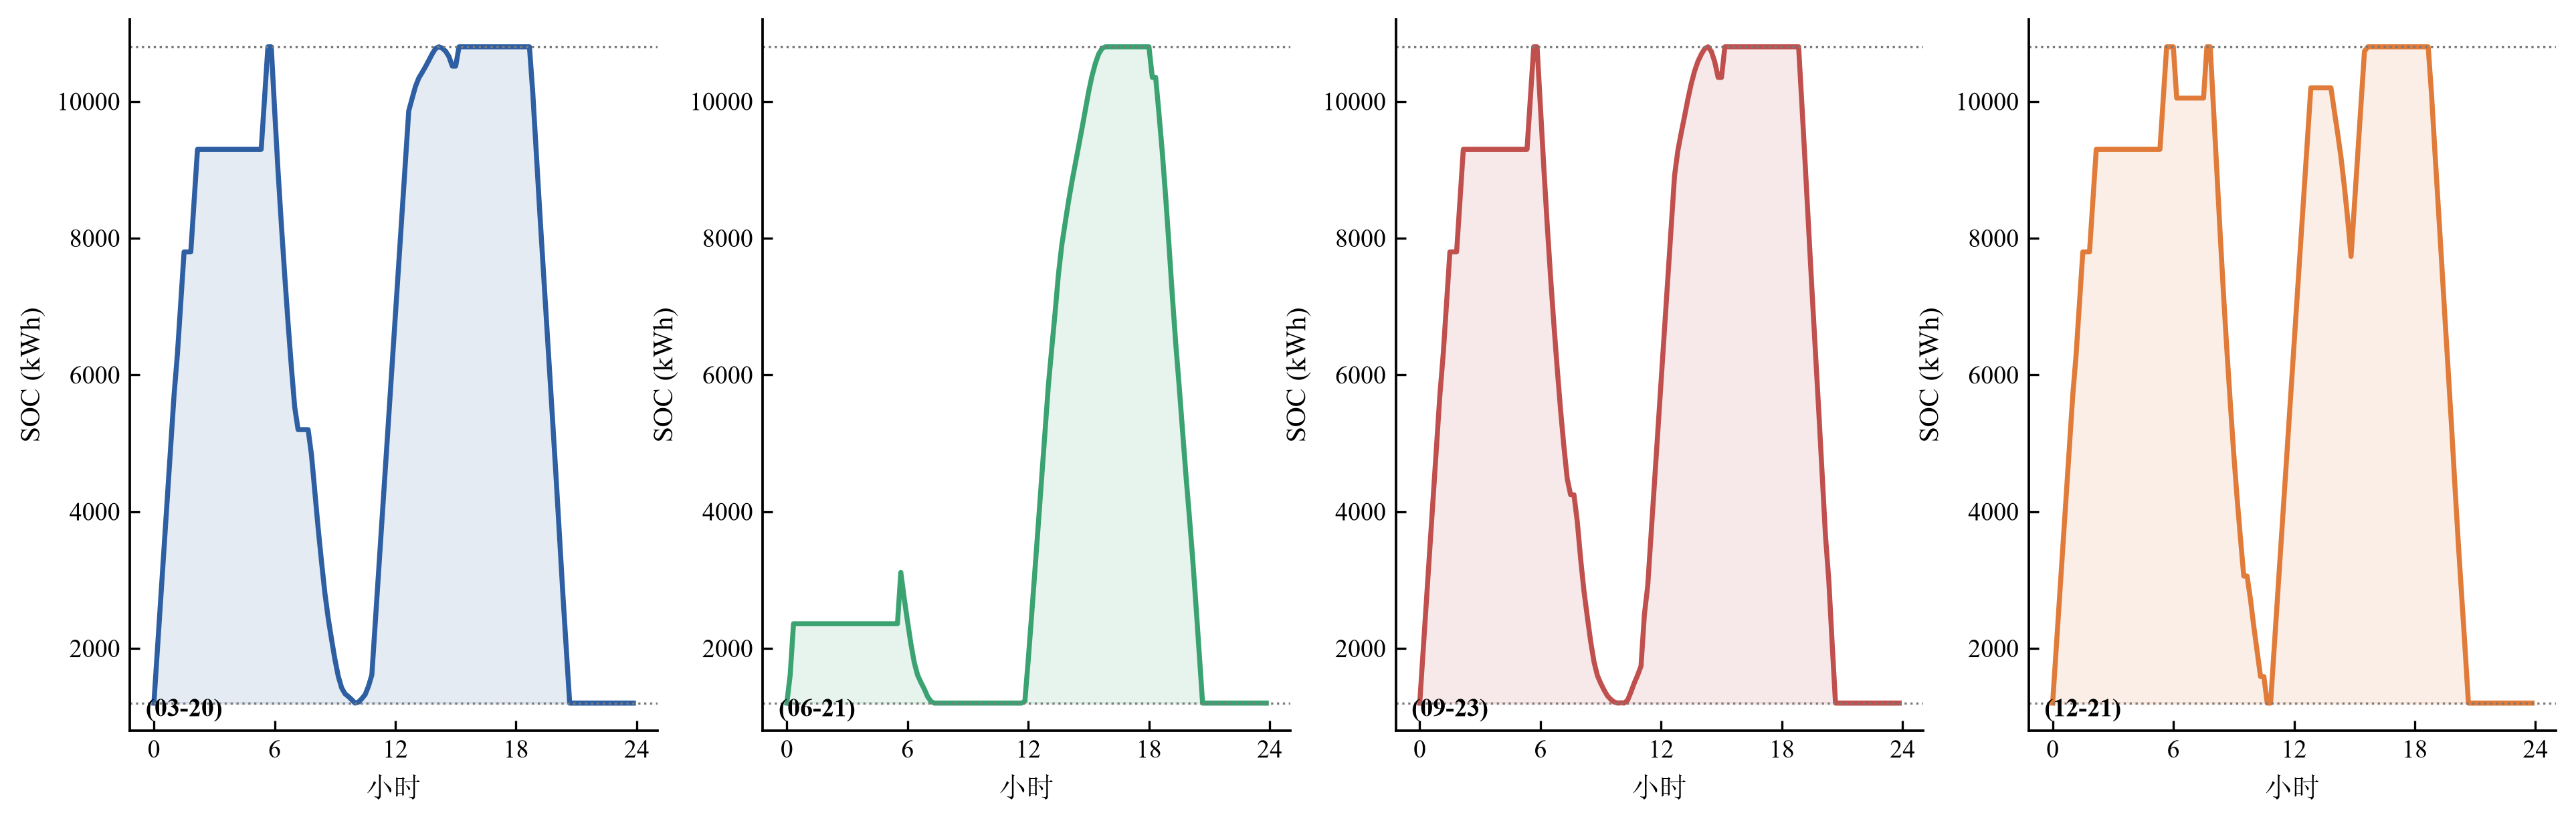
\includegraphics[width=0.75\textwidth]{求解/问题二/图片/图2-4_四季典型日SOC轨迹.png}
    \caption{四季典型日储能荷电状态轨迹}
    \label{fig:结果2-4}
\end{figure}

2—12 月储能每日 0:00 储电量的月度分布如图\ref{fig:结果2-5}所示。各月储电量中位数均处于 1200 kWh 附近，说明储能每日末放至下限的规律在全年保持稳定，符合低充高放套利的最优行为。

\begin{figure}[H]
    \centering
    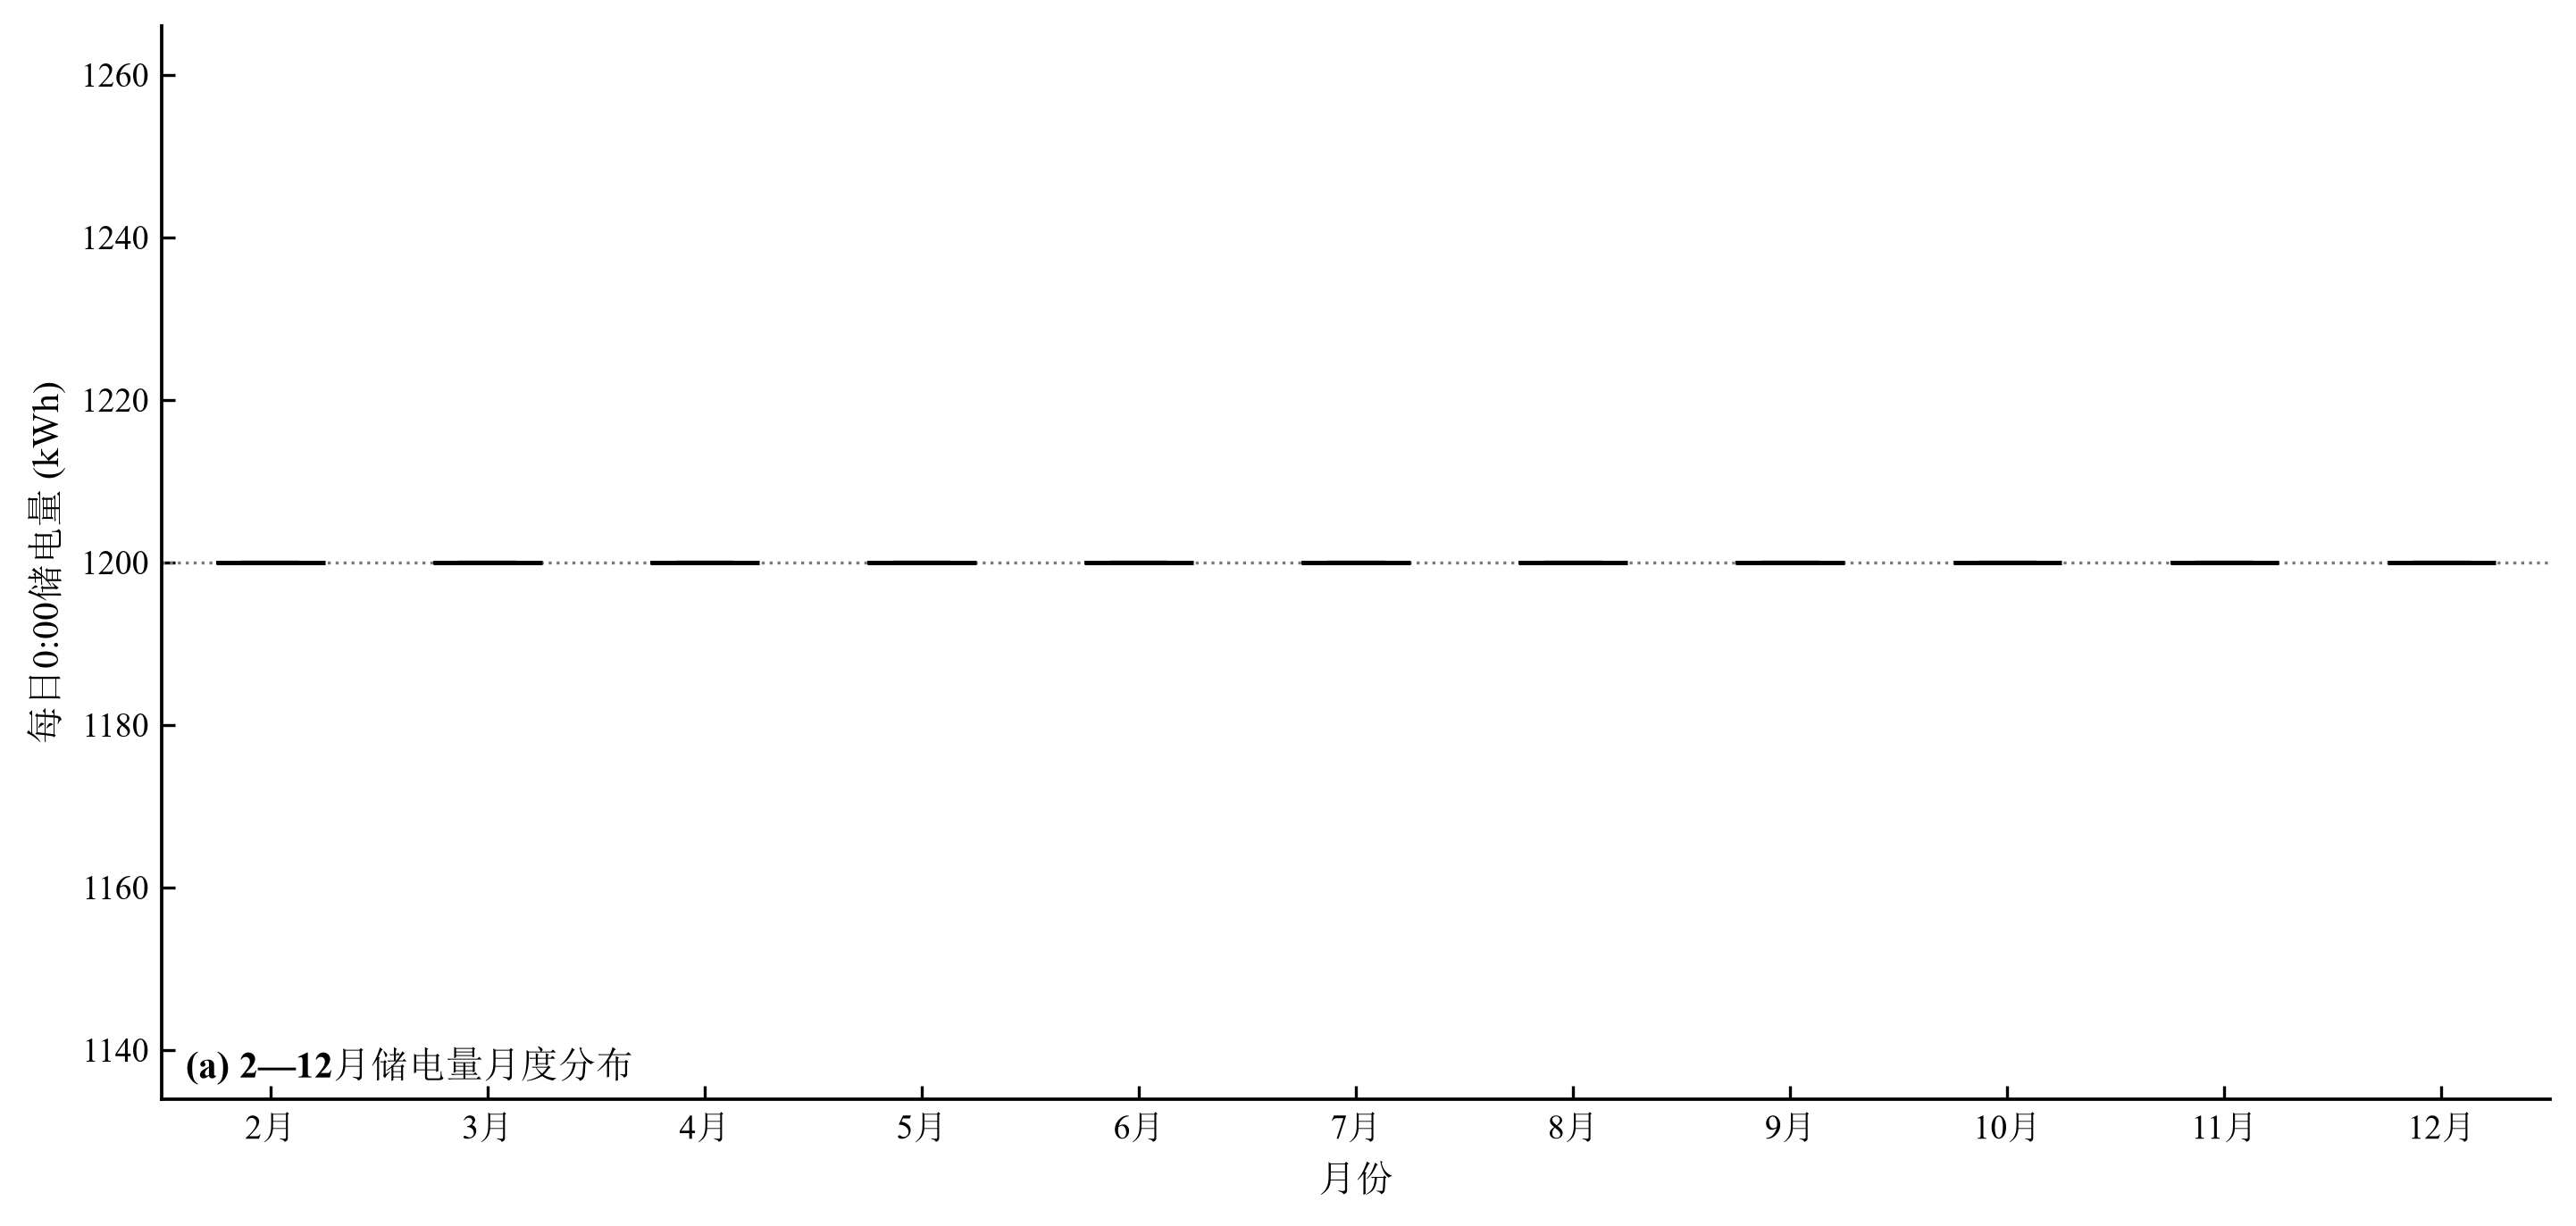
\includegraphics[width=0.70\textwidth]{求解/问题二/图片/图2-5_全年储能SOC月度分布.png}
    \caption{储能每日0:00储电量月度分布（2—12月）}
    \label{fig:结果2-5}
\end{figure}

购电功率与净负荷的关系（2.1—12.31）及月度购电费（2—12月）如图\ref{fig:结果2-6}所示。日均购电功率与日均净负荷呈显著正相关，负荷越大、光伏越小则购电越多；月度购电费在冬季达到峰值、夏季为谷值，进一步印证了模型的合理性。

\begin{figure}[H]
    \centering
    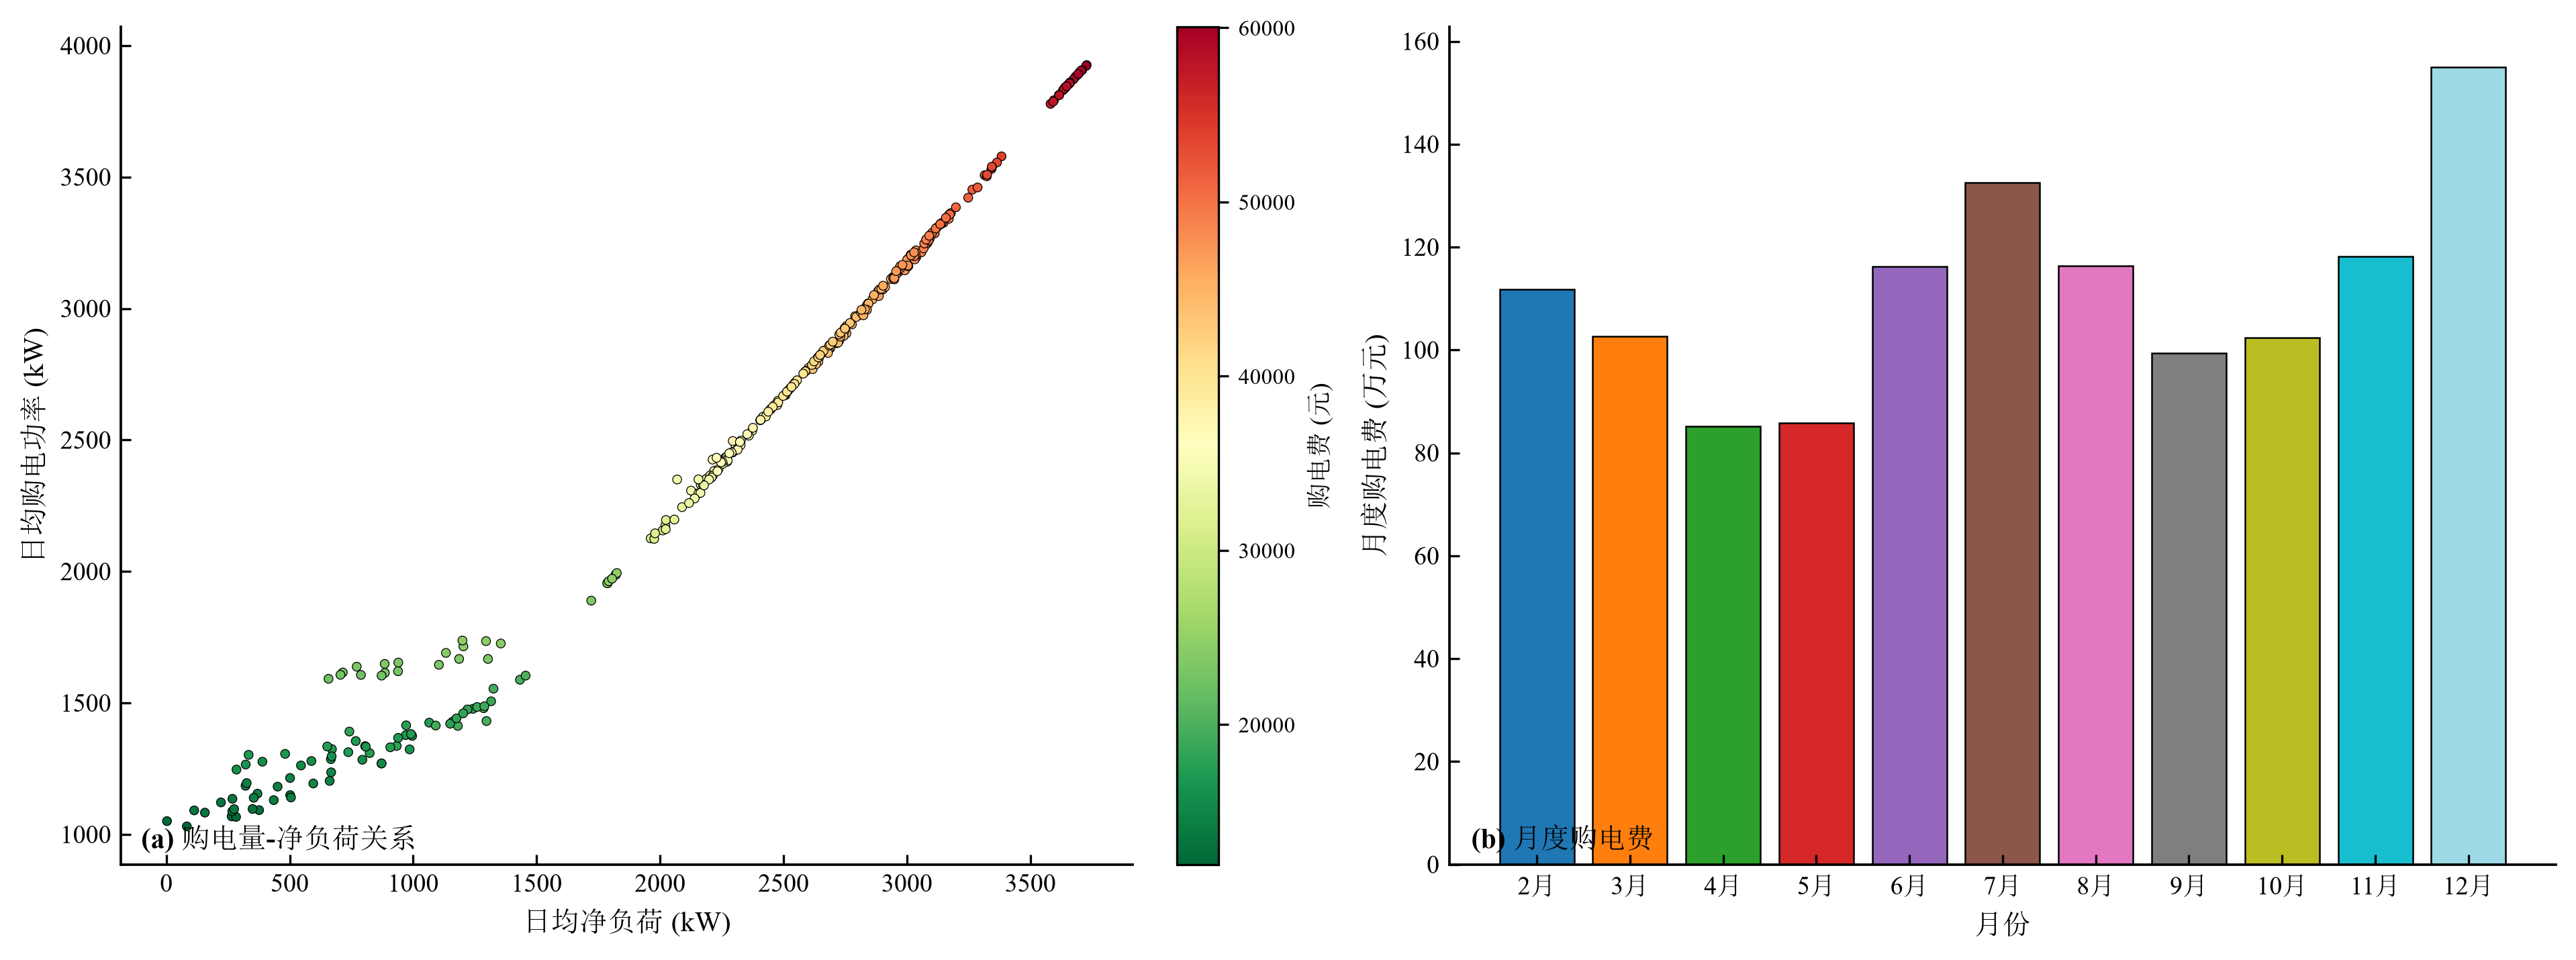
\includegraphics[width=0.72\textwidth]{求解/问题二/图片/图2-6_购电量与净负荷关系.png}
    \caption{购电功率与净负荷的关系及月度购电费}
    \label{fig:结果2-6}
\end{figure}

综合以上结果，问题二的逐日滚动线性规划模型在全年的负载与光伏变化下，通过储能的低充高放显著削减了购电费用，供电缺口恒为零、紧急购电量为零，模型与结果均合理可靠。
